\documentclass[11pt]{beamer}
\usetheme{Warsaw}
\usepackage[utf8]{inputenc}
\usepackage[french]{babel}
\usepackage[T1]{fontenc}
\usepackage{amsmath}
\usepackage{amsfonts}
\usepackage{amssymb}
\usepackage{graphicx}
\usepackage{my_listings}
\usepackage{math}
\usepackage{tikz}
\usepackage{pgfplots}
\author{Théophile \textsc{Bastian}, Noémie \textsc{Cartier}}
\title{Projet d'algorithmique -- Dijkstra}
%\setbeamercovered{transparent} 
\setbeamertemplate{navigation symbols}{}
%\logo{} 
%\institute{} 
\date{8 janvier 2016} 

\pgfplotsset{compat=newest}
\usepgfplotslibrary{units}

\usepackage{xcolor}
\newcommand{\todo}[1]{\colorbox{yellow}{\color{red}#1}}

%\subject{} 
\begin{document}

\begin{frame}
\titlepage
\end{frame}

%\begin{frame}
%\tableofcontents
%\end{frame}

\begin{frame}[fragile]{Dijkstra}
\alert{Idée~:} BFS par distance à l'origine croissante.

\vspace{1em}
\begin{lstlisting}[language=C++]
toProcess = file de priorité min vide
toProcess.insert(origine,0)
dists.fill(-1)
while(not toProcess.isEmpty()) {
	curNode,curDist = toProcess.pop()
	if(dists[curNode] >= 0)
		continue

	dists[curNode] = curDist
	foreach v in voisins[curNode] {
		toProcess.insert(v, curDist + dist[curNode, v])
	}
}
\end{lstlisting}

\alert{Complexité~:} $\bigO\left(\card{E} (Ins(\card{E}) + Pop(\card{E})\right)$.

\end{frame}

\section{Version naïve}

\subsection{Implémentation naïve}
\begin{frame}{Implémentation naïve}
\alert{File de priorité~:} Tableau. Insertion en $\bigO(1)$, suppression en $\bigO(N)$ \\
\qquad $\Longrightarrow$ Dijkstra en $\bigO(\card{E}^2)$.

\vspace{1em}
Nécessite des \alert{tableaux à taille variable}.

\vspace{1em}
\begin{block}{Graphes}
\begin{itemize}
\item Nombre de sommets $\card{V}$ fixe
\item Listes d'adjacence~: tableau de $\card{V}$ tableaux à taille variable de voisins (et le poids de l'arête)
\end{itemize} 
\end{block}
\end{frame}

\section{Tas de Fibonacci}

\subsection{Algorithme}

\begin{frame}{Tas de \textsc{Fibonacci}}
\begin{block}{Complexités}
Insertion~: $\bigO(1)$\\
Suppression~: $\bigO(\log(N))$ (amorti)
\end{block}

\vspace{1em}
\begin{figure}[H]
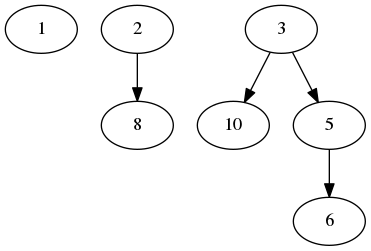
\includegraphics[width=0.6\linewidth]{fiboheap.png}
\end{figure}
\end{frame}

\subsection{Implémentation}

\begin{frame}{Structures nécessaires}
\begin{itemize}
\item Structure d'\alert{arbre}
\item Structure de \alert{liste doublement chaînée cyclique}
\item Structure de \alert{tas de Fibonacci}
\end{itemize}
\end{frame}

\begin{frame}{Arbre}
\begin{itemize}
\item Structure récursive
\item Pointeur \lstc{child}
\item Pointeur \lstc{sibling}
\item Portée des variables $\leadsto$ \lstc{malloc}
\end{itemize}
\end{frame}

\begin{frame}{Liste doublement chaînée cyclique}
\begin{itemize}
\item Pointeurs \lstc{prev}, \lstc{next}
\item Toujours \lstc{malloc}
\item Liste vide~: pointeur sur \lstc{NULL}
\item Gestion du passage de liste non-vide à liste vide et inversement
\item Prendre un pointeur, en renvoyer un presque toujours identique
\item Cycliques~: permet de faciliter leur usage dans les tas de Fibonacci
\end{itemize}
\end{frame}

\begin{frame}{Tas de Fibonacci}
\begin{itemize}
\item \lstc{insert}~: insertion d'un n\oe ud dans la liste
\item \lstc{pop}~: retrait du plus petit n\oe ud de la liste et ajout dans la liste de ses arbres fils~; fusion des arbres de taille identique
\item Quelques difficultés sur la fusion qui n'était pas faite
\end{itemize}
\end{frame}

\section{Correction et performances}

\subsection{Correction}

\begin{frame}{Correction}
\begin{itemize}
\item Résultats vérifiés à la main sur de petits graphes
\item Comparaison entre les deux implémentations et une implémentation de référence C++ utilisant la STL
\item Tests automatisés sur 10000 graphes de grande taille
\item Erreur détectée et corrigée pour des arêtes de poids 0
\item Pas de fuite de mémoire~: \lstbash{valgrind}
\end{itemize}
\end{frame}

\subsection{Performances}

\begin{frame}{Performances}
\begin{itemize}
\item Tests de performance effectués comparant nos deux implémentations sur de très grands graphes aléatoires de taille variable
\item Fibonacci~: quasi-linéaire
\item Naïf~: quadratique
\item Quelques aberrations sur les plus petits graphes, liées à des problèmes de connexité
\end{itemize}
\end{frame}

\begin{frame}{Comparatif -- degrés faibles (1 -- 3)}
\begin{figure}
  \begin{center}                                                                
    \begin{tikzpicture}                                                         
      \begin{axis}[                                                             
          width=\linewidth, % Scale the plot to \linewidth                      
          height=0.65\textwidth, % Scale the plot to \linewidth                 
          grid=major, % Display a grid                                          
          grid style={dashed,gray!30}, % Set the style                          
          xlabel=Nombre de sommets, % Set the labels                            
          ylabel=Temps d'exécution,                                             
          x unit=, % Set the respective units                                   
          y unit= s, %\si{\second},                                                  
          legend style={at={(0.5,-0.2)},anchor=north},                          
          x tick label style={rotate=90,anchor=east}                            
        ]                                                                       
        \addplot table[x=nbVert,y=naive,col sep=tab] {../report/bench_lowdegr.dat} node[above, pos=1] {Naïf};
        \addplot table[x=nbVert,y=opti,col sep=tab] {../report/bench_lowdegr.dat} node[above, pos=1] {Fibonacci};
        \end{axis}                                                              
    \end{tikzpicture}                                                           
    \label{fig:graphlow}                                                        
  \end{center}
\end{figure}
\end{frame}

\begin{frame}{Comparatif -- degrés élevés (0 -- 10)}
\begin{figure}
  \begin{center}                                                                
    \begin{tikzpicture}                                                         
      \begin{axis}[                                                             
          width=\linewidth, % Scale the plot to \linewidth                      
          height=0.65\textwidth, % Scale the plot to \linewidth                 
          grid=major, % Display a grid                                          
          grid style={dashed,gray!30}, % Set the style                          
          xlabel=Nombre de sommets, % Set the labels                            
          ylabel=Temps d'exécution,                                             
          x unit=, % Set the respective units                                   
          y unit= s, %\si{\second},                                                  
          legend style={at={(0.5,-0.2)},anchor=north},                          
          x tick label style={rotate=90,anchor=east}                            
        ]                                                                       
        \addplot table[x=nbVert,y=naive,col sep=tab] {../report/bench_highdegr.dat} node[above, pos=1] {Naïf};
        \addplot table[x=nbVert,y=opti,col sep=tab] {../report/bench_highdegr.dat} node[above, pos=1] {Fibonacci};
        \end{axis}                                                              
    \end{tikzpicture}                                                           
    \caption{Comparaison des temps d'exécution réels -- degrés faibles (1-3)}   
    \label{fig:graphlow}                                                        
  \end{center}
\end{figure}
\end{frame}

\begin{frame}{Fibonacci -- degrés élevés (2 -- 10)}
\begin{figure}
  \begin{center}                                                                
    \begin{tikzpicture}                                                         
      \begin{axis}[                                                             
          width=\linewidth, % Scale the plot to \linewidth                      
          height=0.65\textwidth, % Scale the plot to \linewidth                 
          grid=major, % Display a grid                                          
          grid style={dashed,gray!30}, % Set the style                          
          xlabel=Nombre de sommets, % Set the labels                            
          ylabel=Temps d'exécution,                                             
          x unit=, % Set the respective units                                   
          y unit= s, %\si{\second},                                                  
          legend style={at={(0.5,-0.2)},anchor=north},                          
          x tick label style={rotate=90,anchor=east}                            
        ]
        \addplot table[x=nbVert,y=opti,col sep=tab] {../report/bench_opti.dat} node[above, pos=1] {Fibonacci};
        \end{axis}                                                              
    \end{tikzpicture}                                                           
    \caption{Comparaison des temps d'exécution réels -- degrés faibles (1-3)}   
    \label{fig:graphlow}                                                        
  \end{center}
\end{figure}
\end{frame}

\section{Bonus~: Dijkstra dans Paris}

\subsection{Graphe de Paris~: formatage}

\begin{frame}{Graphe de Paris~: formatage}
\begin{itemize}
\item Données de base~: OpenStreetMaps
\item \alert{Réindexer} les n\oe uds pour avoir des IDs contigus partant de 0
\item Maintenir une table de hachage pour garder la correspondance
\item \alert{Arêtes}~: segments de \lstbash{way} successifs, distance
\[ R_T \sqrt{\left(\Delta \Phi\right)^2 + \left(\cos\left(\Phi_m\right) \Delta \lambda\right)^2} \]
\item Relations (OSM) ignorées
\item Génère deux fichiers~: un graphe \emph{non-orienté} (option adaptée) et un fichier de correspondance des IDs.
\end{itemize}
\end{frame}

\subsection{À une intersection donnée}

\begin{frame}{Vers un lieu donné}
\begin{itemize}
\item Se rendre à l'intersection du \alert{boulevard Brune} et de l'\alert{avenue Jean Moulin} (aka avenue de la Porte de Châtillon)
\item Google maps~: 2.9Km
\item Notre Dijkstra~: 2849m (cohérent)
\item Premier essai sur graphe \alert{orienté}~: 3653m
\end{itemize}
\end{frame}

\begin{frame}{Carte associée}
\begin{figure}
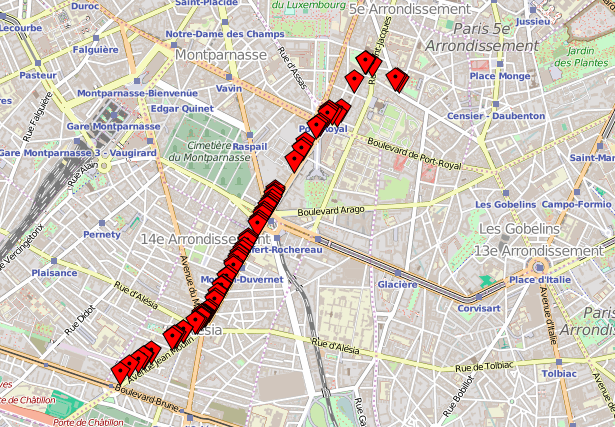
\includegraphics[width=0.9\linewidth]{map1.png}
\end{figure}
\end{frame}

\subsection{Aux lignes RATP}

\begin{frame}{Aux lignes RATP}
\begin{itemize}
\item Récupération des noms, latitude, longitude des stations par ligne
\item Pour chaque ligne, chaque station, trouver tous les nœuds à moins de 50m
\item Lier les station à ces nœuds par leur distance à vol d'oiseau
\item Lier les stations à un nœud \og ligne \fg{} avec poids 0
\item Dijkstra
\item Relier les stations~: naïvement, $\bigO(\text{nbStat} \times \card{V})$. Raffinage du graphe pour supprimer les zones non-connexes.
\end{itemize}
\end{frame}

\begin{frame}{RER A}
\begin{figure}
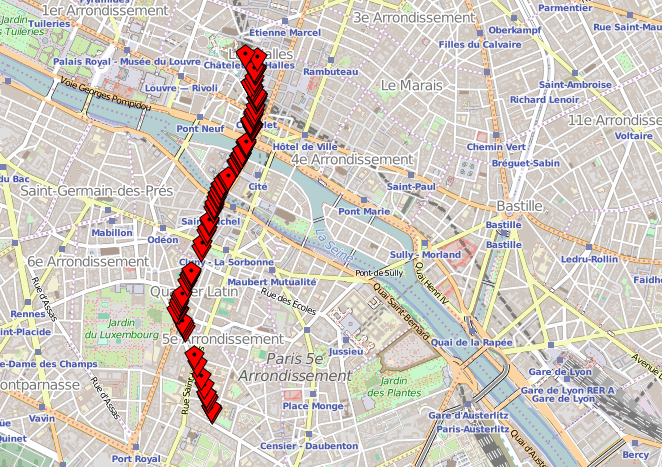
\includegraphics[width=0.9\linewidth]{mapToRerA.png}
\end{figure}
\end{frame}

\section*{}

\begin{frame}{Conclusion}
\begin{itemize}
\item Notre Dijkstra semble marcher sur tous les exemples
\item Si vous voulez prendre la ligne de bus 321, n'y allez pas à pied. 22,848Km, c'est long.
\end{itemize}
\end{frame}

\end{document}